\section{Methodology}
We now describe how we selected our subjects (\secref{sec:sel}) and how we classified their features (\secref{sec:extr}).
 
\subsection{Identification of Subject Environments (RQ1)}
\label{sec:sel}
\looseness=-1
We are interested in environments that support end-user programming of mobile robots. Such environments should provide domain-specific languages for specifying robotic missions (i.e., behaviors and tasks). %Our focus was on environments targeting novice programmers with graphical notations, which we systematically
%We identified the environments from the following data sources  using inclusion and exclusion criteria. 
%\Figref{fig:selection} illustrates how the environments were identified from the following data sources.

%---including languages that are close to the robotics domain---
\looseness=-1
\parhead{Data Sources.}
We used three different data sources: input provided by the authors based on experience and knowledge in the field, the Google search engine, and forward and backward snowballing upon a set of related survey papers.
%These candidates were then filtered based on explicitly formulated inclusion and exclusion criteria (explained shortly).

%Since a web search for ``robot mission'' alone would not return enough relevant results, we designed a systematic search taking into account multiple sources, varying terminologies (programmable robots, robot programming environment or mission specification environment).  and explicitly defined inclusion and exclusion criteria.
%Specifically, our identification process involved data collection to identify environment candidates, then applying inclusion-exclusion criteria to the candidates, and finally identifying alternative environments\tb{not clear to me what the last point means}. 

\parhead{Identification of Candidate Environments.}
As a first step, we identified candidate environments, i.e., software for programming robots mentioned in a source that appeared to fit our study scope; then we identified mobile robots and successively looked for additional candidate environments. Then, we applied inclusion and exclusion criteria.
As shown in \figref{fig:selection} we used the following strategy:
%but before applying dedicated inclusion and exclusion criteria (explained shortly)---using the following strategy.

%\texttt{Step a.}  % -> would be confusing with the three main steps
\emph{Environment candidates from experience.} From our past experience in robotics software engineering, we assembled a list of 25 candidate environments.

%\texttt{Step b.}
\emph{List of mobile robots.} We created a list of 59 commercial mobile robots based on our past experience (e.g., we were aware of many educational robots, such as Thymio, Sphero or NAO) and from conducting a Google search (``mobile robot'').
%were aware of various robot programming environments, which led to 25 environment candidates. 
%The authors also created a list of 59 mobile robots based on experience, each person listing any mobile robots that he knows. \patrizio{then we contribute with our experience two different lists, one of non-commercial environments in the first item, and one of commercial environments in this item. At the beginning of the section we only mention one list. This should be clarified: it's confusing.}
From the robots' web pages, we identified that software that was offered for programming the robot missions, which gave us exactly 59 environment candidates.
%The respective robot websites and Google search using the robot name as search string  were used to identify the environments in which missions are specified for the robots.

%\texttt{Step c.}
\looseness=-1
\emph{Google search.} We conducted a search with the string \emph{(``programmable robots" OR (``robot programming" OR ``mission specification") environment) ``mobile robot"}, which yielded 373 results (note that Google reported 774,000 results%\patrizio{tried now and my results are 52000!! This string: ("programmable robots" OR ("robot programming" OR "mission specification") environment) "mobile robot"}
, which Google search engine collapsed to 373 %\patrizio{138 in my case!}
while omitting some entries very similar in order to show the most relevant results).

%collapsed into 373 when selecting the last page).

%\texttt{Step d.}
\emph{ Snowballing.} Based on a list of six survey papers\,\cite{Biggs2003,Bravo2018,Jost2015,Luckcuck2018,Nordmann2016a,Hentout2017} we were aware of from our experience, we conducted snowballing. Specifically, we identified environment candidates from reading these survey papers and then from reading all papers being cited in each (backwards snowballing) and all papers citing it (forward snowballing), also ignoring duplicates. We identified 12 from \citet{Biggs2003}, 44 from \citet{Bravo2018}, 14 from \citet{Jost2015}, 0 from \citet{Luckcuck2018}, 6 from \citet{Nordmann2016a}, and 7 from \citet{Hentout2017}, totaling 83 candidates.
%Snowballing.
%1.	Six papers were identified
%2.	From each paper, environments were extracted. 
%3.	Forward snowballing: papers which reference the candidate papers were read to extract further environments.
%4.	Backward snowballing: papers in the reference list of the candidate papers were read to extract environments
%•	The environments extracted were then subjected to inclusion and exclusion criteria to generate the final list.
%•	Duplicate environments were removed.

%\claudio{Old}
%\begin{itemize}
 %   \item From our past experience in robotics software engineering, we were aware of various robot programming environments, which led to 25 environment candidates
    %\tb{really so many? I cannot remember that we came up with so many; where's the list?} \swaib{check "validation sheet" in the data collection spreadsheet}\tb{not sure where exactly, but I see sth. with 13. Please give the list to the co-authors in the chat for verification, also put as comments in this Latex file}.
%   \item The authors created a list of 59 mobile robots based on experience, each person listing any mobile robots that he knows. \patrizio{then we contribute with our experience two different lists, one of non-commercial environments in the first item, and one of commercial environments in this item. At the beginning of the section we only mention one list. This should be clarified: it's confusing.}\tb{afair, the list of mobile robots came from experience and a Google search} \tb{still need details}. 
 %   The respective robot websites and Google search using the robot name as search string  were used to identify the environments in which missions are specified for the robots. % \tb{?}\tb{how? I thought you checked the websites; if so, please write}\tb{how many?}.
   %\tb{reference then}
   %\tb{need details}
  %  \item We conducted a Google search with the search string \emph{("programmable robots" OR ("robot programming" OR "mission specification") environment) "mobile robot"}, which yielded 774000 results. However, after scanning through all the web pages returned,
%     \claudio{Did we really do that? 
%     Some calculation: by assuming we spent 10 minutes each it lead to 10750 days... good job! We should be a bit care full.
%     }
%     we found only 373 hits, a common phenomenon with Google search. 
%     \item For snowballing, six survey and review papers were identified on environments and languages.
%     %to \ugh{contact snowball}. \patrizio{if we identified 25 environment candidates in the previous step, why we identified only 6 papers? I would expect at least one paper for each candidate environment.} \swaib{The 6 papers are not specific to one environment and the 25 environments have not gone through inclusion and exclusion criteria}
%     %\ugh{Both forward snowball based on new papers which cite the candidate paper and backward snowball based on papers in the reference list of the candidate paper, were done}.
%     %\patrizio{write in active way, for instance: We performed both forward...} 
%     We performed both forward snowballing based on new papers which cite the candidate papers and backward snowballing based on papers in the reference list of the candidate papers. A total of 83 environments were identified \cite{Biggs2003} 12, \cite{Bravo2018} (44), \cite{Jost2015} (14), \cite{Luckcuck2018} (0), \cite{Nordmann2016a} (6) and \cite{Hentout2017} (7), totalling to 83 candidate environments.\tb{still need more details, incl. how many transitive relations you followed (not sure how this is called exactly in the snowballing literature, but there must be a measure of the number of levels etc.)}
%     \item We lastly used the robots programmed using the environments identified from the above data sources to identify alternative environments for programming them. This was done by doing Google search, with robot name as the search string as shown in \figref{selection}. \claudio{This goes in Section 3.2}
% \end{itemize}  

% \tb{did pass until here in this section}
In summary, we collected 537 candidate environments.

\parhead{Application of Inclusion and Exclusion Criteria.}
In the second step, we filtered the 537 candidates according to the following inclusion and exclusion criteria.

\noindent
 \emph{Inclusion Criteria.} We included a candidate when it fulfilled all of the following conditions. It must:
%\patrizio{be more clear. To be included any of the following should be true, some of them, only one?}
\begin{itemize}
\item allow the specification of missions for mobile robots; 
\item offer a domain-specific language with a visual notation targeting end users; % or a textual notation,
%\item is end-user-facing enabling user domain experts to specify a mission in the environment, 
\item come with documentation about the environment and its language;
\item be available to users in the sense that it is either sold or can be downloaded freely, in other words, has indications of being used by practitioners.
%in table \ref{tablelist} some environments were studied using documentation only. May be we have to remove them or remove the (I,W,D) column in the table. these include \flyaq, \tivipe, \missionlab, \aseba, \codelab, and \choregraphe }
\end{itemize}

\noindent
 \emph{Exclusion Criteria.} 
 An environment is excluded if any of the following conditions holds. It must not either:
\begin{itemize}
\item be an environment that focuses on programming system aspects of a robot, such as the Robotics Operating System (ROS), instead of specifying missions;
%are general purpose, \patrizio{what does it mean general purpose here?}
\item target non-mobile robots, such as stationary industrial robots, 3D printers or Arduino boards; 
%\patrizio{what about movable industrial robots? Should we be more precise, like non-movable industrial robots?}
%\item environments without mission specification aspects, which rather focus on robot architectures~\cite{Nordmann2016},\patrizio{how this differs from the first item - development environments that are not developed to specify robotic missions, but are general purpose ?}
\item be a mission control application with pre-programmed missions;
\item be a remote-control application for mobile robots.
%\patrizio{write better}
%\item the environment's documentation is only a loose collection of web pages, \patrizio{unclear}
%\item the environment should not be only remote control application (e.g., Drone control apps).\patrizio{primarily is ambiguous. How to measure if something is primarily or not? Explain better}
\end{itemize}

In summary, we selected 26 environments using the inclusion/ exclusion criteria from the initial collection of 537.

\parhead{Find Further Alternative Environments.} In a third step, we used the robots programmed using the environments identified from the above data sources to identify alternative environments for programming them. This was done through a Google search with the robot name as the search string.
In summary, we identified 40 robots from the 26 environments selected, which yielded three more environments. As such, our final number of environments identified is 29. \tabref{tab:DataSources} summarizes our results.

\begin{table*}[t]
\caption{Identified environments per step and data source (cf. \secref{sec:sel})}
\label{tab:DataSources}
\vspace{-.4cm}
\begin{smaller}
\begin{threeparttable}
\begin{tabular}{p{7cm}p{10cm}}\\
\toprule
\textsf{data source} & \textsf{identified environments}\\
\midrule
Environments from experience (25 candidates) & \missionlab, \choregraphe, \lego, \sphero, \tivipe, \aseba, \robotmesh, \edison, \makeblock, \trik, \ardublockly, \minibloq, and \flyaq. \\
List of mobile robots (59 candidates) & \picaxe, \openroberta, \arcbotics, \vex, \metabot, \marty, \tello, and \codelab. \\
Google search (373 candidates) & \missionlab, \choregraphe, \lego, \sphero, \tivipe, \aseba, \robotmesh, \edison, \makeblock, \trik, \ardublockly, \minibloq, \flyaq, \picaxe, \openroberta, \arcbotics, \vex, \metabot, \marty, \tello, \codelab,  \blocklyprop, and \ozoblockly.  \\  % -> what did "\codelab. unique" mean?
Snowballing (80 candidates) &  \lego, \missionlab, \aseba, \vex, \choregraphe, \minibloq,  \ozoblockly, \sphero, \tivipe, \openroberta, \trik, \robotmesh, \enchanting, \easyc and \robotc\\ % -> what did "\robotmesh unique" mean?
Further alternative environments\tnote{1}& \turtlebot, \makeblock, \scratchev \\
\bottomrule
\end{tabular}
\begin{tablenotes}
\item[1] Found by seeking alternative environments for robots supported by the identified environments above
\end{tablenotes}
\end{threeparttable} 
\end{smaller}
\end{table*}
%13 from the team:\missionlab, \choregraphe, \lego, \sphero, \tivipe, \aseba, \robotmesh, \edison, \makeblock, \trik, \ardublockly, \minibloq and \flyaq.  8 environments from mobile robot list: \picaxe, \openroberta, \arcbotics, \vex, \metabot, \marty, \tello, and \codelab.   Interestingly all the 21 from stage 1 and stage 2 were included in stage 3 plus 2 more: \blocklyprop, and \ozoblockly.  Stage 4 generated 15 environments, out of which 12 already exist in stage 3: the exclusive 3 are: \enchanting, \easyc and \robotc.  From alternative environments for robots, 3 selected are: \turtlebot, \makecode, and \scratchev. 

    \begin{figure}[t]
      \centering
      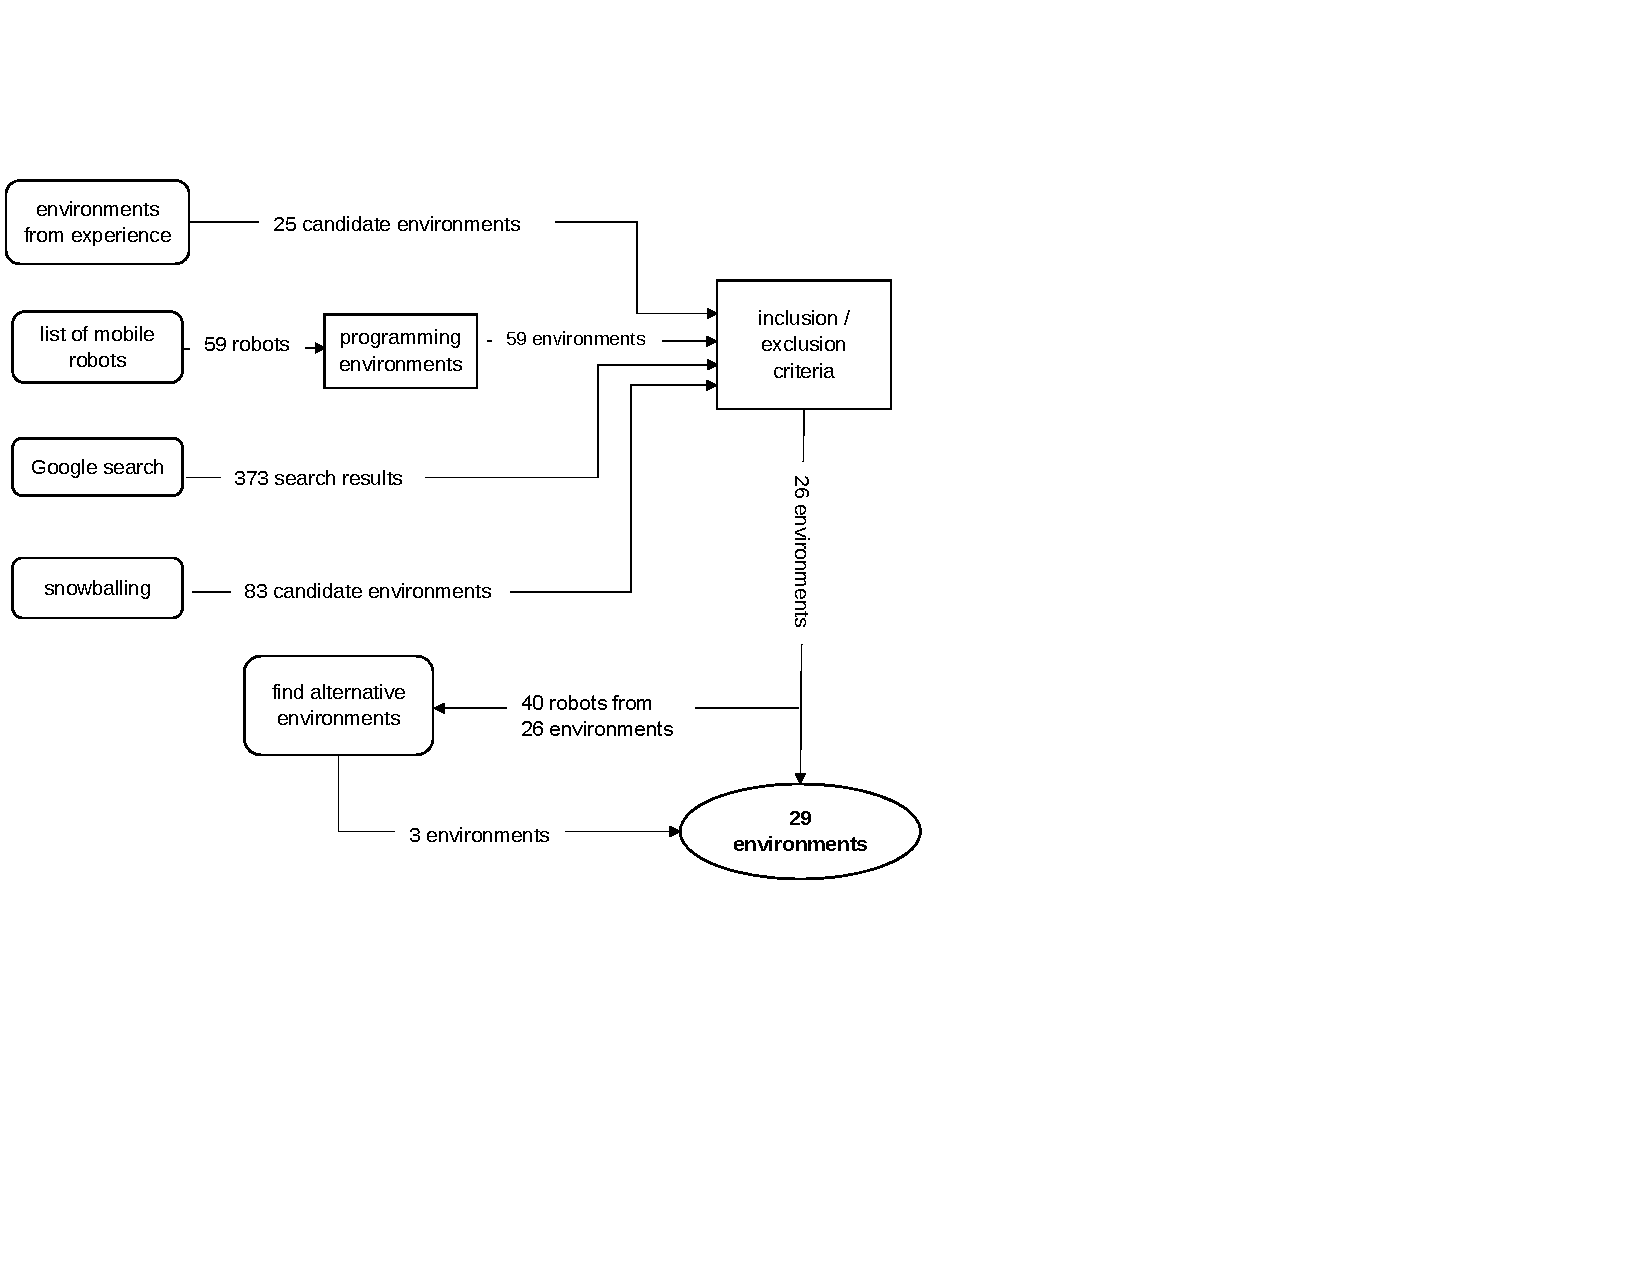
\includegraphics[width=\columnwidth]{fig/selection.pdf}
      %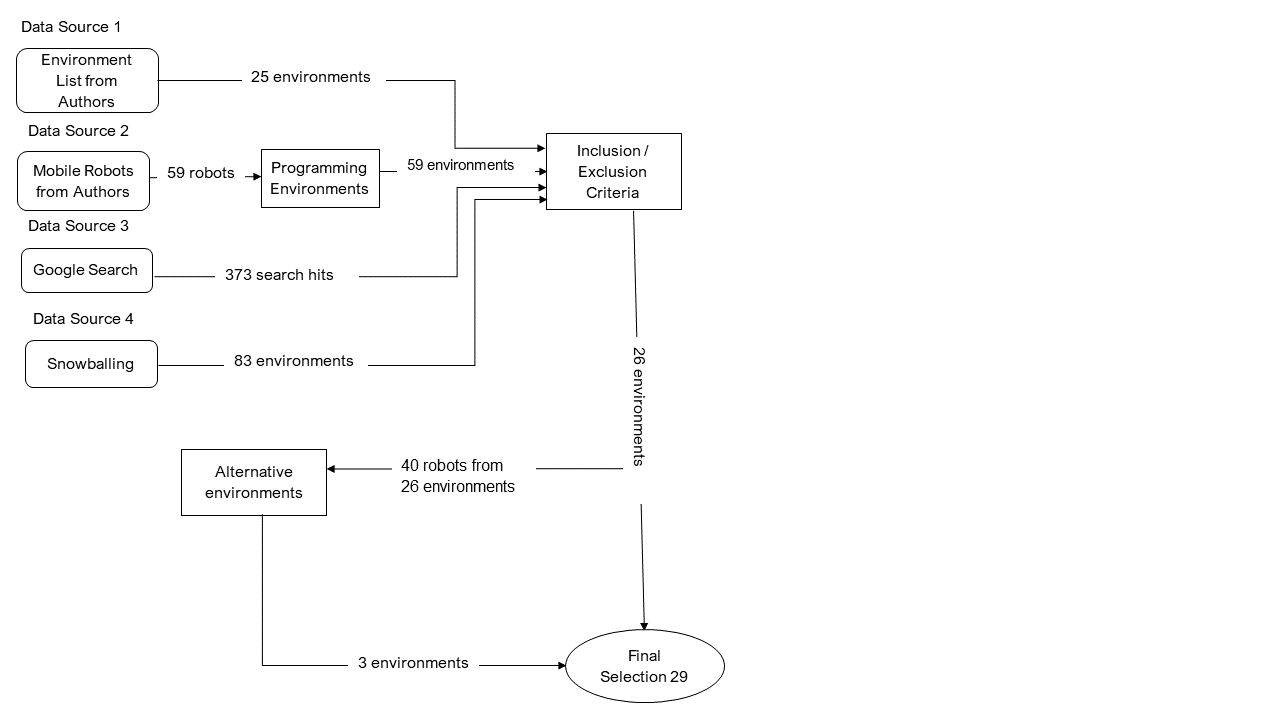
\includegraphics[width=\linewidth]{selection10.png}
      \caption{Identification of subject environments}
      \label{fig:selection}
			\vspace{-.4cm}
    \end{figure}
    

\subsection{Analysis of Identified Environments (RQ2)}
\label{sec:extr}
Our goal is to identify the characteristics that distinguish our subjects in the form of features\,\cite{berger2015feature} and to organize them in a feature model\,\cite{kang.ea:1990:foda,damir2019principles}. Performing such a feature-based analysis is a common method for comparing the design space of technologies, such as model transformations\,\cite{transformationSurvey}, language workbenches\,\cite{erdweg2013languageworkbenches} or variation control systems\,\cite{linsbauer2017gpce}.

The data sources for analyzing the identified environments are scientific papers about them, their websites, related documentation (e.g., user manuals or programming guides), and examples of missions expressed in the respective language.

 %Features were extracted from papers published on selected environments, environment websites, related documentations and  specification of sample missions. We used indirect data collection where researcher did not interact with the participants in this case the environment developers. The data collection technique was independent since the author only accessed the artifacts like publications, specification environments and related websites to extract data for the study\,\cite{Lethbridge2008}. The following steps were followed to extract features from the selected subjects:
%\begin{enumerate}

Our strategy is as follows.
First, in a brainstorming meeting, after an initial screening of the subjects, we identified key features of the environments---mainly representing the top-level and intermediate features in the feature model. Second, we consulted the websites to further identify key features and organize them in a hierarchy. This first skeleton provided the basis for an iterative refinement of the feature model by systematically, for each environment: (i) reading the scientific publications and other technical documentations about the environment; (ii) when possible, downloading and installing the environment to specify example missions, or alternatively for web-based environments, using the online tooling; and (iii) reading through the help menu for better understanding of how the environments are used to specify missions.

\looseness=-1
In this process, we iteratively refined the feature model and maintained a spreadsheet with notes about the realization of the individual features in each environment. The features were discussed among all authors to reach consensus.

%which were then confirmed and refined by an observational study of the selected environments. The brainstorming question used was: ``what mission specification features can be observed in mission specification environments?". 

%(b) General features were extracted from the respective environment websites. 
%
%(c) Read publications and other technical documentations about the environment. 
%
%(d) Downloaded and installed the environments to specify sample missions. Examples for web-based environments were run online.  
%
%(e) Read through the help menu for better understanding of how the environments are used to specify missions.
%The data was collected in a spreadsheet, then analyzed to construct the feature model. 
%%\claudio{Something about how features are connected} \swaib{some hint on how features are connected!}

%\subsection{How research questions were answered}
%\label{sec:answ}
%\noindent
%To answer RQ1, we collected data from multiple sources; teams suggested environments they knew, using mobile robot list we searched for their respective environments in which they are programmed. Snowballing was also done to identify environments mentioned in literature and Google search was also done to identified environments. Using the inclusion \& exclusion criteria we selected 29 environments, which we considered as end-user facing mission specification environments for the study.  RQ2 was answered by identifying features from: literature on selected environments, technical documentation and running sample missions in the environments. The resulting features were tabulated in a spreadsheet. 
